\section{Résumé du projet}
\label{sec:sumup}

\subsection{Contexte}
\label{ssec:contexte}

    À notre époque, assurer la sécurité des systèmes (informatiques ou non) est un enjeu majeur. De nombreuses méthodes de modélisation et d'analyse des systèmes ont donc été développées, dans le but d'identifier les risques et de les quantifier. C'est ainsi que le concept d'ADTrees\footnote{Abréviation d'\og Attack-Defense Trees \fg{}, ou \og Arbres d'Attaque et de Défense\fg{} en français.}~\cite{ADTrees}, un formalisme permettant de représenter sous forme d'arbre les étapes d'une attaque précise contre un système, a vu le jour. L'un des logiciels modélisant ces ADTrees s'appelle ADTool~\cite{ADToolPP}.

    ADTool implémente la plupart des fonctionnalités d'édition d'ADTrees, y compris l'utilisation de paramètres tels que le coût d'une attaque. Mais il a été conçu comme un logiciel de modélisation avant tout, et comporte donc peu d'outils permettant d'analyser les ADTrees.

\subsection{Objectifs}
\label{ssec:objectifs}

    L'objectif de ce projet a donc été la réalisation d'un logiciel fournissant à l'utilisateur, un expert en sécurité, des outils d'analyse des ADTrees. Ce logiciel a été nommé \glasir{} en référence à l'arbre aux feuilles d'or de la mythologie nordique~\cite{vikingCulture}, et dont le logo est visible sur la \textsc{Figure} \ref{fig:glasir}. Il dispose de trois fonctionnalités principales, qui ont été détaillées dans les rapports précédents :
\begin{itemize}
    	\item l'{\bf Éditeur de fonctions}, qui permet à l'expert de créer de nouveaux paramètres fonctions de ceux déjà présents dans l'arbre ;
    	\item le {\bf Filtre}, qui aide l'utilisateur à ôter de l'ADTree les branches dont les valuations ne respectent pas un certain critère;
    	\item l'{\bf Optimiseur}, qui sélectionne le(s) meilleur(s) chemin(s) de l'ADTree selon un paramètre donné.
\end{itemize} 
    ADTool a quant à lui été amélioré, et est utilisé au sein de Glasir comme viewer d'ADTrees. 

\subsection{Bilan}
\label{ssec:bilan}

 \begin{table}[H]
        \centering
        \begin{tabular}{|c|l|c|}
            \hline
            \textbf{Logiciel concerné} & \textbf{Cahier des charges} & \textbf{Implémentation}\\
            \hline
            \multirow{8}{*}{\textbf{Glasir}} & Éditeur de fonctions & \textcolor{bo_vert}{\ding{51}}\\
                    \cline{2-3}
                    & Filtre & \textcolor{bo_vert}{\ding{51}}\\
                    \cline{2-3}
                    & Optimiseur & \textcolor{bo_vert}{\ding{51}}\\
                    \cline{2-3}
                    & Interface graphique & \textcolor{bo_vert}{\ding{51}}\\
                    \cline{2-3}
                     & Gestion des fichiers projets & \textcolor{bo_vert}{\ding{51}}\\
                    \cline{2-3}
                     & Intégration ADTool dans Glasir & \textcolor{nouvo_rouge}{\ding{55}}\\
                    \cline{2-3}
                     & Affichage d'instances multiples d'ADTool & \textcolor{bo_vert}{\ding{51}}\\
                     \cline{2-3}
                     & Bibliothèque de modèles & \textcolor{bo_vert}{\ding{51}}\\
            \hline
            \multirow{4}{*}{\textbf{ADTool}} & Amélioration de la représentation textuelle & \textcolor{bo_vert}{\ding{51}}\\
                    \cline{2-3}
                     & Affichage multi-paramètres & \textcolor{nouvo_rouge}{\ding{55}}\\
                     \cline{2-3}
                     & Copier/couper/coller & \textcolor{bo_vert}{\ding{51}}\\
                     \cline{2-3}
                     & Annulation de l'action précédente & \textcolor{bo_vert}{\ding{51}}\\
            \hline
        \end{tabular}
        \caption{Retour sur le cahier des charges de Glasir.}
        \label{fig:bilan_cdc}
    \end{table}

Il est d'ores et déjà possible de dresser un premier bilan du projet, sous la forme d'une rétrospective sur les éléments définies dans le cahier des charges. Ce premier bilan est présenté sous la forme de la {\sc table}~\ref{fig:bilan_cdc}.

    La 1\iere{} colonne de la {\sc table}~\ref{fig:bilan_cdc} rappelle le cahier des charges tel qu'il a été défini dans le rapport de planification~\cite{planif}, c'est-à-dire sous forme de tâches unitaires. La 2\ieme{} colonne de la {\sc table}~\ref{fig:bilan_cdc} indique si la tâche correspondante a bien été effectuée (symbole \textcolor{bo_vert}{\ding{51}}) ou non (symbole \textcolor{nouvo_rouge}{\ding{55}}). Comme la {\sc table}~\ref{fig:bilan_cdc} permet de le voir, la plupart des fonctionnalités promises dans le cahier des charges du projet ont effectivement été livrées. Il est à noter que si les fonctionnalités implémentées sont fonctionnelles et rendent bien le service décrit initialement dans le cahier des charges, leur implémentation a parfois différé de leur conception pour des raisons pratiques. Ces différences seront détaillées et justifiées par la suite dans la {\sc section}~\ref{sec:rect}.

    Quatre rapports ont été rédigés dans le cadre de ce projet : celui de pré-étude~\cite{pre_etude}, celui de spécifications fonctionnelles~\cite{spec_fonc}, celui de planification~\cite{planif} et celui de conception~\cite{conception}. Ils ont permis de mieux définir les objectifs du logiciel, ainsi que l'organisation de son implémentation. Le but de ce rapport final est de rendre compte de la tenue des objectifs qui ont été fixés au début du projet, et des méthodes mises en place pour y parvenir. Il évoquera aussi les ajustements qui ont été mis en place afin de gérer les imprévus auquels nous avons fait face. 

    Pour cela, ce rapport est composé d'une collection de documents indépendants couvrant l'ensemble de ces aspects : rectificatifs de conception, compte-rendus de tests, description des livrables, manuel des logiciels, et pour finir une rétrospective sur la conduite du projet.

    \vspace{4mm}

    \begin{figure}[!h]
        \centering
        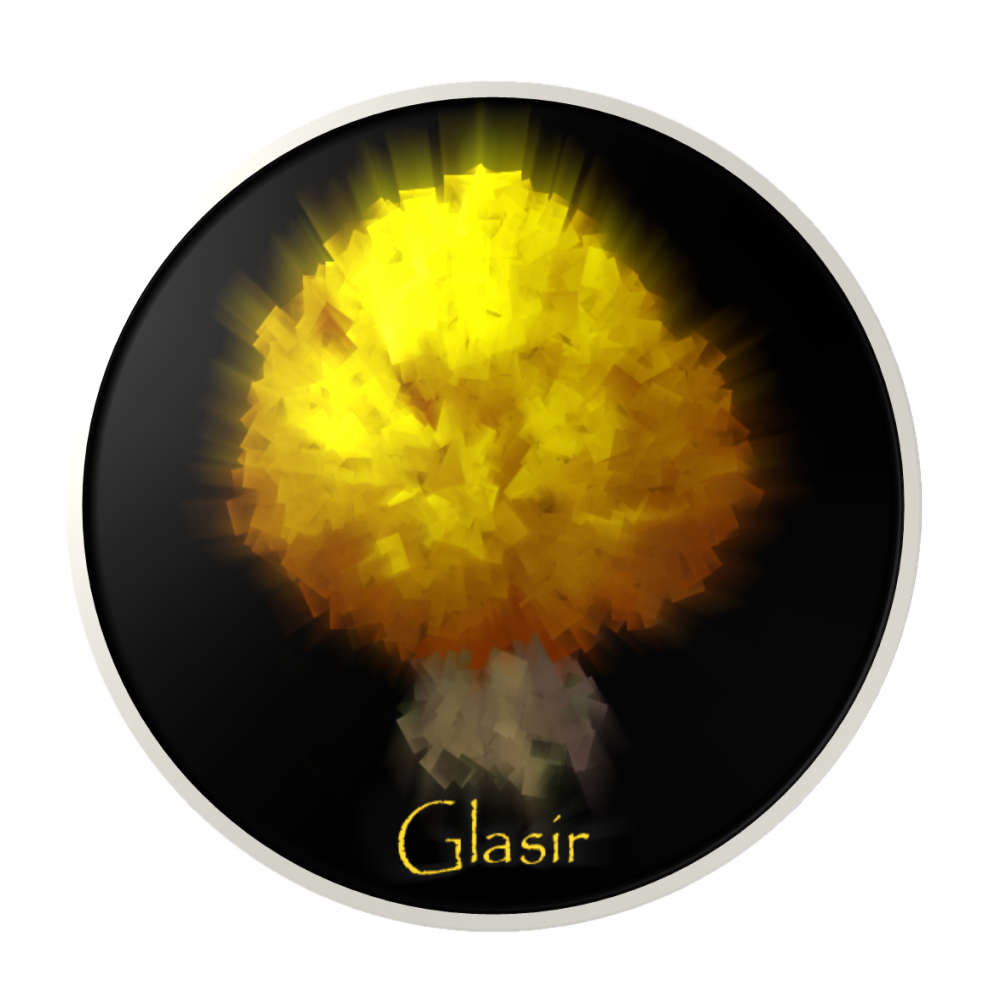
\includegraphics[height=0.5\textwidth]{figure/glasir.png}
        \caption{Logo du logiciel Glasir.}
        \label{fig:glasir}
    \end{figure}